\documentclass[11pt]{article}

\usepackage{amsmath}
\usepackage{amssymb}

\usepackage{graphicx}
\usepackage{tikz}

\usepackage[all]{xy}

\begin{document}


\begin{center}
{\bf Math 4990: Intro to combinatorics and graph theory \\
Fall 2020, Sam Hopkins \\
Midterm exam 2- Due Tuesday Nov. 17th}
\end{center}

\thispagestyle{empty}

{\bf Instructions}: There are 5 problems, worth 20 points each, totaling 100 points. This is an open book, open library, open notes, open web, take-home exam, but you are not allowed to to interact with anyone (including online forums) except for me, the instructor. As always, in order to earn points you need to carefully \emph{explain your answer}.

\begin{enumerate}

\item (20 points) In how many ways can one color $n$ distinct objects (labeled $1,2,\ldots,n$) with $3$ colors, if each color must be used at least once? (Your answer should be expressed as a function of $n$.)

\item (20 points) Define the sequence of numbers $P_0,P_1,P_2,\ldots$ via initial conditions $P_0 = 0$, $P_1 =1$, and recurrence relation $P_{n}=2P_{n-1}+P_{n-2}$ for $n\geq 2$. Find $\displaystyle \lim_{n \to \infty} \frac{P_{n+1}}{P_{n}}$.

\item (20 points) A \emph{rooted plane tree} is a rooted tree drawn in the plane such that the children of each parent vertex are ordered left-to-right. For example, the following are the $5$ rooted plane trees with $4$ vertices:
\[\rotatebox{180}{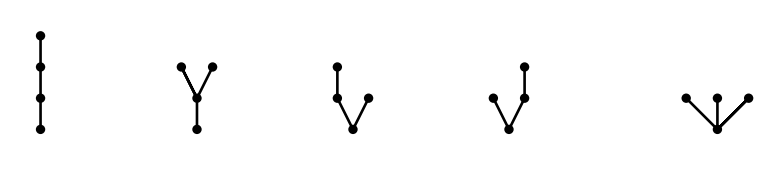
\includegraphics[width=3in]{rooted_plane_trees.png}}\]
Let $D_n$ denote the number of rooted plane trees with $n+1$ vertices. Show that these number satisfy the Catalan number recurrence, i.e., that $D_{n+1} = \sum_{k=0}^{n} D_{k}D_{n-k}$.

\item (20 points total) The \emph{complete bipartite graph} $K_{n,n}$ is the simple graph with $2n$ vertices $x_1,x_2,\ldots,x_n,y_1,y_2,\ldots,y_n$ and $n^2$ edges $\{x_i,y_j\}$ for $1 \leq i,j \leq n$. (The $x_i$ aren't adjacent to each other; ditto for the $y_j$.) 
\begin{enumerate}
\item (10 points) For which values of $n$ does $K_{n,n}$ have an Eulerian circuit? Justify your answer.
\item (10 points) For which values of $n$ does $K_{n,n}$ have a Hamiltonian cycle? Justify your answer.
\end{enumerate}

\item (20 points) A \emph{leaf} of a tree is a vertex of degree one. Show that a tree that has at least one vertex of degree $d$ has at least $d$ leaves.

\end{enumerate}


\end{document}
